% document setup
\documentclass{article}
\usepackage[left=0.7in, right=0.7in, top=0.7in, bottom=0.7in]{geometry}
\usepackage{fancyhdr}
\usepackage[utf8]{inputenc}
\usepackage[english]{babel}

% fonts
\usepackage[T1]{fontenc}
\usepackage[osf]{libertine}
\usepackage[scaled=0.8]{beramono}

% packages
\usepackage{url}
\usepackage{multirow}
\usepackage{array}
\usepackage{booktabs}
\usepackage{microtype}
\usepackage{caption}
\usepackage{float}
\usepackage{stmaryrd}
\usepackage[shortlabels]{enumitem}
\usepackage{graphicx}
\graphicspath{{/}}

% math packages
\usepackage{amsmath}
\usepackage{amsfonts}
\usepackage{amssymb}
\usepackage{graphicx}
\usepackage{mathtools}
\usepackage{nicefrac}
%\usepackage{minted}
\usepackage{algorithm}
\usepackage[noend]{algpseudocode}
\usepackage{tikz}
\usepackage{tikz-qtree}

% plotting 
\usepackage{pgfplots}
\pgfplotsset{
  compat=newest,
  plot coordinates/math parser=false,
  tick label style={font=\footnotesize, /pgf/number format/fixed},
  label style={font=\small},
  legend style={font=\small},
  every axis/.append style={
    tick align=outside,
    clip mode=individual,
    scaled ticks=false,
    thick,
    tick style={semithick, black}
  }
}

% custom math operators
\DeclareMathOperator*{\argmin}{\arg\!\min}
\DeclareMathOperator{\E}{\mathbb{E}}
\DeclarePairedDelimiter\floor{\lfloor}{\rfloor}
\renewcommand{\vec}[1]{\mathbf{#1}} % overriding vector
\newtheorem{theorem}{Theorem}[section]
\newtheorem{lemma}[theorem]{Lemma}
\newtheorem{conj}[theorem]{Conjecture}

% page setup
\pagestyle{fancy}
\fancyhf{}
\lhead{\textbf{Left Head}}
\chead{\textbf{Center Head}}
\rhead{\textbf{Section \thesection}}
\setlength\parindent{0pt} 

\begin{document}

\section{Section Heading}
\subsection{Subsection Heading}
\subsubsection{Subsubsection Heading}

\section{Maths}
\subsection{Operators}
\subsubsection{argmin}
$$\argmin_{x}{f(x)}$$

\subsubsection{Expected value}
$$\E[X] = \int{xp(x)dx}$$

\subsubsection{Floor operator}
$$\floor{x+y}$$

\subsubsection{Vector modifier}
$$c\vec{X} + d\vec{y}$$

\subsection{Diagrams}
\subsubsection{Small Tables}
\begin{table}[H]
  \centering
    \hspace*{-4em}\begin{tabular}{*{6}{c|}}
      \multicolumn{2}{c}{} & \multicolumn{4}{c}{Player LJ} \\
      \cline{3-6}
      \multicolumn{1}{c}{} & & {(w,w)} & {(w,c)} & {(c,w)} & {(c,c)} \\
      \cline{2-6}
      \multirow{2}{*}{Player BJ} & w & 0,0 & 0,0 & \color{red}9,1 & \color{red}9,1 \\
      \cline{2-6}
      & c & \color{red}4,4 & 5,3 & 4,4 & 5,3 \\
      \cline{2-6}
    \end{tabular}
    \caption{Normal form representation}
\end{table}

\subsubsection{Trees}
\begin{center}
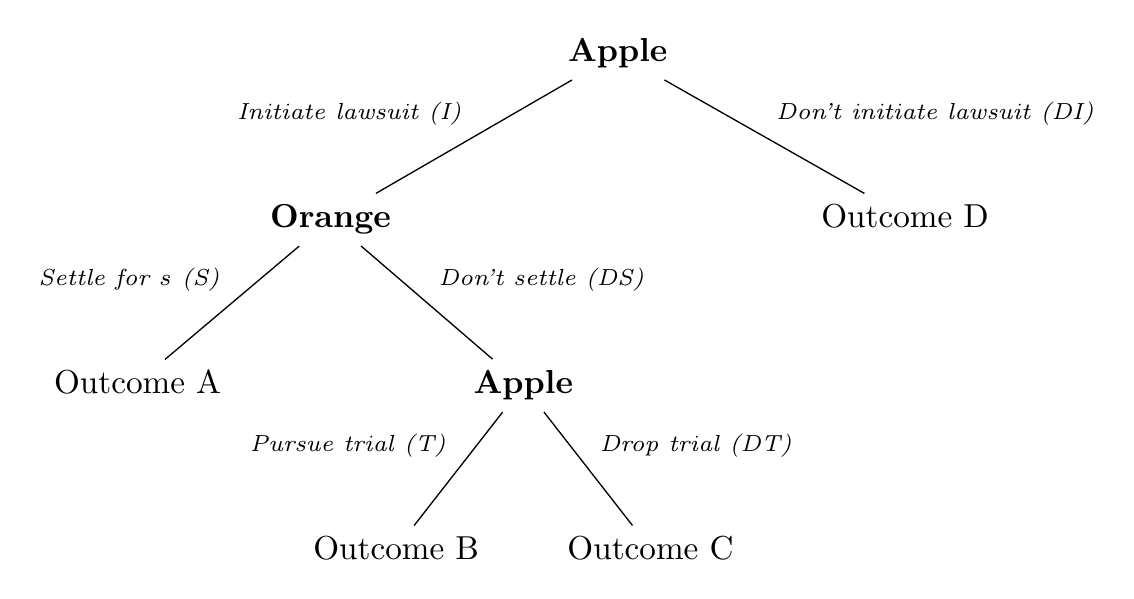
\begin{tikzpicture}[
  thin,
  scale=1.2,
  edge from parent path={(\tikzparentnode) -- (\tikzchildnode)},
  level distance=50pt,
  level 3/.style={sibling distance=20pt}
]
  \Tree [ .\textbf{Apple}
          \edge node[auto=right] {\textit{\scriptsize Initiate lawsuit (I)}};
          [ .\textbf{Orange}
            \edge node[auto=right] {\textit{\scriptsize Settle for $s$ (S)}};
             [ .{Outcome A} ]
            \edge node[auto=left] {\textit{\scriptsize Don't settle (DS)}};
            [ .\textbf{Apple}
              \edge node[auto=right] {\textit{\scriptsize Pursue trial (T)}};
              [ .{Outcome B} ]
              \edge node[auto=left] {\textit{\scriptsize Drop trial (DT)}};
              [ .{Outcome C} ]
            ]
          ]
          \edge node[auto=left] {\textit{\scriptsize Don't initiate lawsuit (DI)}};
          [ .{Outcome D} ]
        ]
\end{tikzpicture}
\end{center}

\section{Document improvements}
\subsection{Lists}
\begin{enumerate}[(a)]
  \item A first item
  \item A second item
  \item A third item
\end{enumerate}

\subsection{Tables}
\begin{tabular}{rrrrrrrr} \toprule
    {$m$} & {$\Re\{\underline{\mathfrak{X}}(m)\}$} & {$-\Im\{\underline{\mathfrak{X}}(m)\}$} & {$\mathfrak{X}(m)$} & {$\frac{\mathfrak{X}(m)}{23}$} & {$A_m$} & {$\varphi(m)\ /\ ^{\circ}$} & {$\varphi_m\ /\ ^{\circ}$} \\ \midrule
    1  & 16.128 & +8.872 & 16.128 & 1.402 & 1.373 & -146.6 & -137.6 \\
    2  & 3.442  & -2.509 & 3.442  & 0.299 & 0.343 & 133.2  & 152.4  \\
    3  & 1.826  & -0.363 & 1.826  & 0.159 & 0.119 & 168.5  & -161.1 \\
    4  & 0.993  & -0.429 & 0.993  & 0.086 & 0.08  & 25.6   & 90     \\ \midrule
    5  & 1.29   & +0.099 & 1.29   & 0.112 & 0.097 & -175.6 & -114.7 \\
    6  & 0.483  & -0.183 & 0.483  & 0.042 & 0.063 & 22.3   & 122.5  \\
    7  & 0.766  & -0.475 & 0.766  & 0.067 & 0.039 & 141.6  & -122   \\
    8  & 0.624  & +0.365 & 0.624  & 0.054 & 0.04  & -35.7  & 90     \\ \midrule
    9  & 0.641  & -0.466 & 0.641  & 0.056 & 0.045 & 133.3  & -106.3 \\
    10 & 0.45   & +0.421 & 0.45   & 0.039 & 0.034 & -69.4  & 110.9  \\
    11 & 0.598  & -0.597 & 0.598  & 0.052 & 0.025 & 92.3   & -109.3 \\ \bottomrule
\end{tabular}

\end{document}